\section{Operacje na węzłach}
W tej sekcji poznamy sposoby otrzymywania nowych obiektów z~już istniejących (rewers i~lustro splotu).
Rodzina węzłów wyposażona w~sumę spójną tworzy przemienny monoid z~jednoznacznością rozkładu.
Znacznie później (w sekcji \ref{sec:tangle}) określimy jeszcze sumę oraz iloczyn supłów.


\subsection{Lustro i~rewers. Węzły skrętne i zwierciadlane}
\begin{definition}[lustro]
% DICTIONARY;mirror;lustro/lustrzany;węzeł
\index{lustro}%
\index{węzeł!lustrzany}% TODO: to się może mylić ze zwieciadlanym
    Niech $L$ będzie zorientowanym splotem.
    Splot $mL$ powstały przez odbicie splotu $L$ względem dowolnej płaszczyzny nazywamy lustrem.
\end{definition}

\begin{definition}[rewers]
% DICTIONARY;reverse;rewers/odwrotny;węzeł
\index{rewers}%
\index{węzeł!odwrotny}%
    Niech $L$ będzie zorientowanym splotem.
    Splot $rL$ powstały przez odwrócenie orientacji wszystkich ogniw splotu $L$ nazywamy rewersem.
\end{definition}

\begin{comment}
\begin{figure}[H]
    \begin{minipage}[b]{.32\linewidth}
        \centering
        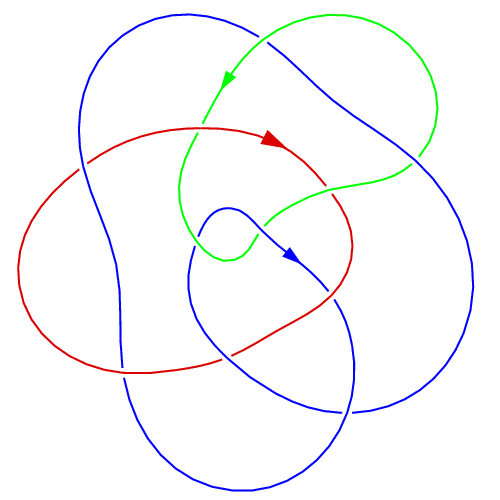
\includegraphics[width=\linewidth]{../data/link_mirror.png}
        \subcaption{lustro $mL$}
    \end{minipage}
    \begin{minipage}[b]{.32\linewidth}
        \centering
        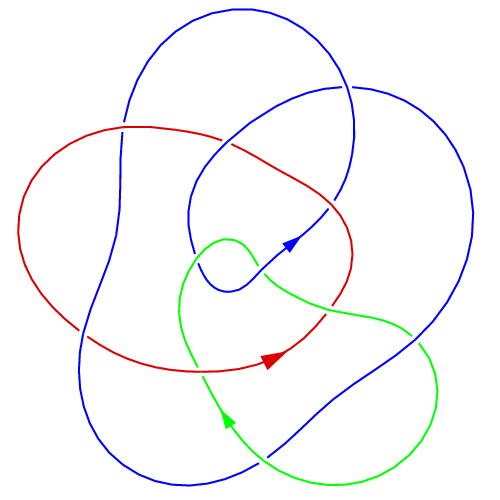
\includegraphics[width=\linewidth]{../data/link.png}
        \subcaption{przykładowy splot $L$}
    \end{minipage}
    \begin{minipage}[b]{.32\linewidth}
        \centering
        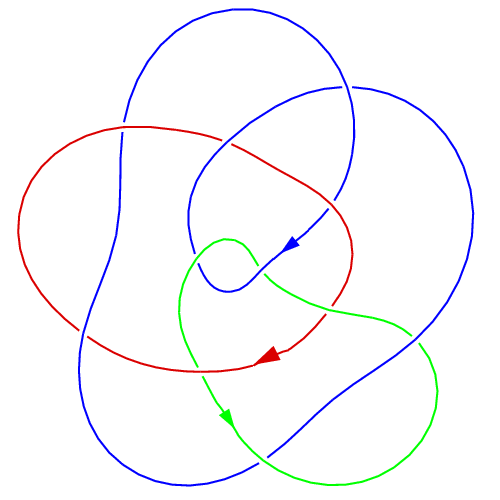
\includegraphics[width=\linewidth]{../data/link_reverse.png}
        \subcaption{rewers $rL$}
    \end{minipage}
\end{figure}
\end{comment}

Na lewym obrazku odbiliśmy diagram względem poziomej prostej, innym sposobem na otrzymanie lustra jest odwrócenie wszystkich skrzyżowań, co odpowiada odbijaniu względem płaszczyzny papieru.
Zauważmy, że wykonując powyższe operacje na węźle możemy otrzymać mniej niż czterech różne obiekty ($L$, $mL$, $rL$, $mrL$) -- na przykład trójlistnik jest własnym rewersem, ale nie lustrem.

Wyróżniamy pięć typów symetrii węzłów:

% DICTIONARY;chiral;skrętny/chiralny;węzeł
\begin{definition}[całkowicie chiralny albo skrętny]
\index{węzeł!chiralny}%
\index{węzeł!skrętny|see {węzeł lustrzany}}%
    Węzły $K$, $rK$, $mK$ są parami nierównoważne. % chiral 9_32
\end{definition}

% DICTIONARY;reversible;odwracalny;węzeł
\begin{definition}[odwracalny]
    \index{węzeł!odwracalny}%
    Węzły $K \cong rK$ są równoważne. % reversible 3_1
\end{definition}

% DICTIONARY;achiral/amphicheiral;zwierciadlany;węzeł
\begin{definition}[zwierciadlany ujemnie]
    \index{węzeł!zwierciadlany}%
    Węzły $K \cong mrK$ są równoważne. % negative amphicheiral 8_17
\end{definition}

\begin{definition}[zwierciadlany dodatnio]
    Węzły $K \cong mK$ są równoważne. % positive amphicheiral 12a_427
\end{definition}

\begin{definition}[całkowicie zwierciadlany]
    Węzły $K, rK, mK$ są parami równoważne. % fully amphicheiral 4_1
\end{definition}

\begin{example}
    Węzeł $9_{32}$ jest całkowicie skrętny.
\end{example}

% Całkowicie skrętne są też między innymi wszystkie węzły torusowe.
% TODO: wiki pisze Each nontrivial torus knot is prime[4] and chiral.[2]

\begin{example}
    \label{exm:trefoil_is_chiral}
    Trójlistnik jest odwracalny, ale nie zwierciadlany.
\end{example}

Po raz pierwszy odkrył to Max Dehn w 1914 roku \cite{dehn14}.
Oto, jak tego dokonał.
% równik = equator
% równoleżnik = parallel (of latitude), najdłuższy równoleżnik to równik
% południk = meridian (of longitude)
% https://math.stackexchange.com/questions/2511364/how-did-dehn-prove-that-the-trefoil-is-chiral myli te pojęcia: pisze o meridian i longitude, kiedy oryginalna praca Dehna operowała na longitude i latitude
Iloraz grafu Cayleya dla grupy podstawowej trójlistnika, $G = \pi_1(S^3 - K)$, zanurza się w~produkt $\mathbb H^2 \times \R$, co pozwala wyznaczyć grupę zewnętrznych automorfizmów grupy $G$, $\Z/2\Z$.
\index{grupa!podstawowa}
% DICTIONARY;latitude;szerokość geograficzna;geografia
% DICTIONARY;longitude;długość geograficzna;geografia
% DICTIONARY;meridian (of longitude);południk;geografia
% DICTIONARY;parallel (of latitude);równoleżnik;geografia
% DICTIONARY;---;geografia;-
Korzystając z~południków i~równoleżników pokazał następnie, że nietrywialny automorfizm zewnętrzny odwraca orientację przestrzeni otaczającej.

My przekonamy się o~tym po wyznaczeniu wielomianu Jonesa trójlistnika, patrz wniosek \ref{cor:joines_of_amphicheiral}.

\begin{example}
    Węzeł $8_{17}$ jest zwierciadlany ujemnie, ale nie odwracalny.
\end{example}

Sześćdziesiąt lat temu matematycy nie byli pewni, czy węzły nieodwracalne w~ogóle istnieją \cite[problem 10]{fox62};
obecnie wiadomo, że nieodwracalne są prawie wszystkie węzły (Murasugi \cite[s.~46]{murasugi96}).
\index[persons]{Murasugi, Kunio}%
W~roku 1962 Ralph Fox wskazał kilku kandydatów do tego tytułu.
\index[persons]{Fox, Ralph}%
Hale Trotter odkrył rok później nieskończoną rodzinę nieodwracalnych precli, patrz \ref{prp:pretzel_not_invertible}.
\index[persons]{Trotter, Hale}%

% MAKOTO SAKUMA - A SURVEY OF THE IMPACT OF THURSTON’S WORK ON KNOT THEORY
% Hartley [129] realized that one can apply this method to the problem of identifying noninvertible knots, as follows. Suppose no automorphism of Γ maps γ to γ−1. Then the set R(G(K), Γ, γ) is possibly different from the set R(G(K), Γ, γ−1), and there is a chance to show noninvertibility of K by comparing the homology invariants associated with φ ∈ R(G(K), Γ, γ) with those associated with φ′ ∈ R(G(K), Γ, γ−1). Hartley showed that this method is quite effective: he completely determined the 36 non-invertible knots up to 10 crossings claimed by Conway to be noninvertible.

\begin{example}
    Węzeł $12a_{427}$ jest zwierciadlany dodatnio, ale nie odwracalny.
\end{example}

Żaden inny węzeł pierwszy o mniej niż 13 skrzyżowaniach nie ma tej cechy.

\begin{example}
\label{property_of_eight_knot}%
    Ósemka $4_1$ jest całkowicie zwierciadlana.
\end{example}

To najprostszy typ symetrii, wystarczy jawnie wskazać przekształcenie między diagramem węzła, jego lustra oraz odwrotności.

Tait odnosił wrażenie, że zwierciadlane węzły mają parzysty indeks skrzyżowań, ale Hoste, Thistlethwaite znaleźli w~1998 kontrprzykład o~piętnastu skrzyżowaniach, $15_{700}$. % wg https://mathworld.wolfram.com/AmphichiralKnot.html
(Czwarta) hipoteza Taita jest prawdziwa dla węzłów pierwszych, alternujących.

\begin{proposition}[10.4.4 w \cite{kawauchi96}, \ref{cor:joines_of_amphicheiral} u nas]
    Niech $K$ będzie węzłem zwierciadlanym.
    Wtedy
    \begin{align}
        V(t) & = V(1/t) \\
        P(a, z) & = P(1/a, z) \\
        F(a, z) & = F(1/a, z),
    \end{align}
    gdzie $\jones, P, F$ oznacza kolejno wielomian Jonesa, HOMFLY oraz Kauffmana.
    Równość $\conway(z) = \conway(-z)$ zachodzi dla wszystkich węzłów, zwierciadlanych lub nie.
\end{proposition}

Poniższa tabela oparta jest (kolejno) o~ciągi
\href{https://oeis.org/A051766}{51766},
\href{https://oeis.org/A051769}{51769},
\href{https://oeis.org/A051768}{51768},
\href{https://oeis.org/A051767}{51767},
\href{https://oeis.org/A052400}{52400},
z bazy danych ``The On-Line Encyclopedia of Integer Sequences'' (OEIS).

\begin{table}[h]
    \centering
    \begin{tabular}{@{}*{20}l@{}} \toprule
        skrzyżowania & 3 & 4 & 5 & 6 & 7 & 8 & 9 & 10 & 11 & 12 & 13 & 14 \\ \midrule
        całkowicie skrętne & 0 & 0 & 0 & 0 & 0 & 0 & 2 & 27 & 187 & 1103 & 6919 & 37885 \\
        odwracalne & 1 & 0 & 2 & 2 & 7 & 16 & 47 & 125 & 365 & 1015 & 3069 & 8813 \\
        $-$ zwierciadlane & 0 & 0 & 0 & 0 & 0 & 1 & 0 & 6 & 0 & 40 & 0 & 227 \\
        $+$ zwierciadlane & 0 & 0 & 0 & 0 & 0 & 0 & 0 & 0 & 0 & 1 & 0 & 6 \\
        zwierciadlane & 0 & 1 & 0 & 1 & 0 & 4 & 0 & 7 & 0 & 17 & 0 & 41 \\
        \bottomrule
        \hline
    \end{tabular}
    \caption{Liczba węzłów o~poszczególnych typach symetrii}
\end{table}

\begin{definition}[10.3.2 w \cite{kawauchi96}]
    Niech $K \subseteq S^3$ będzie węzłem.
    Jeśli istnieje inwolucja pary $(S^3, K)$, która zachowuje orientację sfery, ale odwraca orientację węzła, to węzeł $K$ nazywamy silnie odwracalnym.
\end{definition}

\begin{proposition}
    Jeśli węzeł jest silnie odwracalny, to jest też odwracalny.
    Implikacja odwrotna nie zachodzi.
\end{proposition}

Hipotezę, że implikacja odwrotna jednak zachodzi, postawił Montesinos \cite[problem 1.6]{kirby78}, on też zdefiniował klasę silnie odwracalnych węzłów \cite{montesinos75}.
\index[persons]{Montesinos, José}%

\begin{proof}
\index[persons]{Hartley, Richard}%
\index[persons]{Whitten, Wilbur}%
    Pierwsza część jest oczywista.
    Hartley \cite{hartley80} oraz Whitten \cite{whitten81} niezależnie od siebie zaproponowali kontrprzykłady do implikacji odwrotnej.
\end{proof}

Ale hiperboliczny węzeł odwracalny jest silnie odwracalny.
% Kawauchi bez dowodu.

\begin{proposition}
    Każdy wielomian Alexandera jest realizowany przez pewien silnie odwracalny węzeł.
\end{proposition}

\begin{proof}
\index[persons]{Sakai, Tsuyoshi}%
    Sakai konstruuje w \cite{sakai83} silnie odwracalny węzeł o dowolnie wybranym cyklicznym module Alexandera.
\end{proof}

% Koniec podsekcji Lustro i rewers




\subsection{Węzły okresowe}
\index{węzeł!okresowy|(}%
Można wyróżnić jeszcze jeden rodzaj symetrii.

% DICTIONARY;period;okres;-
% DICTIONARY;periodic;okresowy;węzeł
\begin{definition}
\label{def:period}%
    Węzeł $K$ nazywamy $n$-okresowym, jeśli istnieje obrót $f \colon \R^3 \to \R^3$ o~kąt $2\pi/n$ wokół pewnej prostej $l$, rozłącznej z~węzłem, taki że $f(K) = K$.
\end{definition}

Zamiast obrotów można rozpatrywać dowolne odwzorowania okresowe $f \colon S^3 \to S^3$, których zbiór punktów stałych jest rozłączny z węzłem $K$, homeomorficzny z $S^1$ oraz które trzymają węzeł $K$ w miejscu, ale dostaje się wtedy dokładnie taką samą klasę węzłów.
\index{hipoteza!Smitha}
Wynika to z hipotezy Smitha, otrzymanej z połączenia głębokich teorii dotyczących geometrii i topologii 3-rozmaitości.
% Kawauchi, ćwiczenie 10.1.10
% Morgan-Bass 1984

\begin{proposition}
    Zbiór wszystkich okresów jest niezmiennikiem węzłów.
\end{proposition}

Nieodwracalny węzeł $8_{17}$ nie posiada żadnych okresów.
% ćwiczenie 10.1.5 w Kawauchi
Węzeł $5_1$ 5-okresowy, co widać na standardowym diagramie, oraz 2-okresowy, tę drugą symetrię można dostrzec na diagramie realizującym indeks mostowy.
Trójlistnik ma dokładnie dwa okresy, $2$ i~$3$.
Ogólniej, jak głosi Kawauchi \cite[ćwiczenie 10.1.9]{kawauchi96}:

\begin{proposition}
    Jedynymi okresami węzła $(p, q)$-torusowego są dzielniki liczb $p$ oraz $q$.
\end{proposition}

Z~każdym węzłem okresowym związany jest inny, prostszy węzeł.
Niech $f$ będzie obrotem z definicji \ref{def:period}, zaś $p \colon \R^3 \to \R^3/f \simeq \R^3$ rzutem na przestrzeń ilorazową.
% DICTIONARY;quotient;ilorazowy;węzeł
\index{węzeł!ilorazowy}%
Wtedy $p(K)$ nazywamy \emph{węzłem ilorazowym}, zaś $K$ to jego $n$-krotne nakrycie.

Murasugi podał dwa warunki, które musi spełniać węzeł o~okresie $n = p^r$, gdzie $r$ jest liczbą pierwszą.
Do ich zrozumienia potrzebujemy prostej definicji.
Ustalmy półprostą, która nie jest styczna do węzła $K$, po czym zorientujmy ją oraz węzeł.
Indeksem zaczepienia $\lambda$ węzła $p(K)$ jest różnica między liczbą skrzyżowań dodatnich oraz ujemnych wzdłuż półprostej (bez znaku).

\begin{proposition}[warunek Murasugiego]
\index{warunek Murasugiego}%
\label{prp:murasugi_periodic}%
    Niech $K$ będzie węzłem o~okresie $n = p^r$, gdzie $p$ jest liczbą pierwszą.
    Niech $J$ będzie jego węzłem ilorazowym, z~indeksem zaczepienia $\lambda$.
    Wtedy wielomian $\alexander_J$ jest dzielnikiem wielomianu $\alexander_K$ oraz istnieje pewna całkowita liczba $k$, taka że
    \begin{equation}
        \alexander_K(t) \equiv \pm t^k \alexander_J(n)^n \left(1 + t + t^2 + \ldots + t^{\lambda - 1}\right)^{n-1} \mod p.
    \end{equation}
\end{proposition}

\begin{proof}
    Mozolne operacje na macierzach, których wyznacznikiem jest wielomian Alexandera, patrz \cite{murasugi71}.
    Kawauchi przedstawia inny dowód: najpierw dowodzi tego dla węzła torusowego $T_{n, d}$, którego węzłem ilorazowym jest niewęzeł.
    W ogólnym przypadku, korzysta z relacji kłębiastej dla wielomianu Conwaya.
    Szczegóły oraz odsyłacze do dalszych prac znaleźć można w jego przeglądowej publikacji \cite[s. 122-124]{kawauchi96}.
\end{proof}

\index{węzeł!okresowy|(}%

% koniec podsekcji Węzły okresowe




\subsection{Suma niespójna i~suma spójna}

\begin{definition}[suma niespójna]
% DICTIONARY;distant union;suma niespójna;-
\index{suma niespójna}%
    Niech $L_1$ oraz $L_2$ będą splotami, które leżą po różnych stronach ustalonej płaszczyzny w przestrzeni $\R^3$.
    Teoriomnogościową sumę $L_1 \sqcup L_2$ nazywamy sumą niespójną splotów.
\end{definition}

\begin{definition}[suma spójna]
% DICTIONARY;connected sum;suma spójna;-
\index{suma spójna}%
    Niech $K_1, K_2$ będą zorientowanymi węzłami.
    Natnijmy każdy z nich w dwóch punktach tego samego krótkiego łuku, a następnie zszyjmy dwoma łukami, które nie przecinają już istniejących, jak na obrazku.
    Otrzymany węzeł nazywamy sumą spójną węzłów $K_1$ oraz $K_2$ i oznaczamy przez $K_1 \shrap K_2$.
\begin{comment}
    \[
        \begin{tikzpicture}[baseline=-0.65ex,scale=0.09]
        \useasboundingbox (-12, -15) rectangle (12, 10);
        \begin{knot}[clip width=5, flip crossing/.list={5}, ignore endpoint intersections=false,]
            \strand[thick] (-3.5, -3.5) [in=down, out=up] to (3.5, 3.5);
            \strand[thick] (3.5, 3.5) [in=right, out=up] to (-4.5, 10);
            \strand[thick] (-4.5, 10) [in=up, out=left] to (-10, 3.5);
            \strand[thick] (-10, 3.5) to (-10, -3.5);
            \strand[thick] (-10, -3.5) [in=left, out=down] to (-4.5, -10);
            \strand[thick] (-4.5, -10) [in=down, out=right] to (3.5, -3.5);
            \strand[thick] (3.5, -3.5) [in=down, out=up] to (-3.5, 3.5);
            \strand[thick] (-3.5, 3.5) [in=left, out=up] to (4.5, 10);
            \strand[thick] (4.5, 10) [in=up, out=right] to (10, 3.5);
            \strand[thick, -Latex] (10, 3.5) to (10, -3.5);
            \strand[thick] (10, -3.5) [in=right, out=down] to (4.5, -10);
            \strand[thick] (4.5, -10) [in=down, out=left] to (-3.5, -3.5);
            \node at (0, -15) {$K_1$};
        \end{knot}
        \end{tikzpicture}
        \shrap
        \begin{tikzpicture}[baseline=-0.65ex,scale=0.09]
        \useasboundingbox (-12, -15) rectangle (12, 10);
        \begin{knot}[clip width=5, flip crossing/.list={6}, ignore endpoint intersections=false,]
            \strand[thick] (-3.5, -3.5) [in=down, out=up] to (3.5, 3.5);
            %\strand[thick] (3.5, 3.5) [in=right, out=up] to (-4.5, 10);
            %\strand[thick] (-4.5, 10) [in=up, out=left] to (-10, 3.5);
            \strand[thick] (-10, -3.5) [in=left, out=up] to (0, 6.5);
            \strand[thick, Latex-] (-10, -3.5) [in=left, out=down] to (-4.5, -10);
            \strand[thick] (-4.5, -10) [in=down, out=right] to (3.5, -3.5);
            \strand[thick] (3.5, -3.5) [in=down, out=up] to (-3.5, 3.5);
            %\strand[thick] (-3.5, 3.5) [in=left, out=up] to (4.5, 10);
            %\strand[thick] (4.5, 10) [in=up, out=right] to (10, 3.5);
            \strand[thick] (10, -3.5) [in=right, out=up] to (0, 6.5);
            \strand[thick] (10, -3.5) [in=right, out=down] to (4.5, -10);
            \strand[thick] (4.5, -10) [in=down, out=left] to (-3.5, -3.5);
            %
            \strand[thick] (-3.5, 3.5) [in=left, out=up] to (0, 10);
            \strand[thick] (3.5, 3.5) [in=right, out=up] to (0, 10);
            \node at (0, -15) {$K_2$};
        \end{knot}
        \end{tikzpicture}
        =
        \begin{tikzpicture}[baseline=-0.65ex,scale=0.09]
        \useasboundingbox (-27, -15) rectangle (27, 10);
        \begin{knot}[clip width=5, flip crossing/.list={5, 22, 23}, ignore endpoint intersections=false,]
            \strand[thick] (-18.5, -3.5) [in=down, out=up] to (-11.5, 3.5);
            \strand[thick] (-11.5, 3.5) [in=right, out=up] to (-19.5, 10);
            \strand[thick] (-19.5, 10) [in=up, out=left] to (-25, 3.5);
            \strand[thick] (-25, 3.5) to (-25, -3.5);
            \strand[thick] (-25, -3.5) [in=left, out=down] to (-19.5, -10);
            \strand[thick] (-19.5, -10) [in=down, out=right] to (-11.5, -3.5);
            \strand[thick] (-11.5, -3.5) [in=down, out=up] to (-18.5, 3.5);
            \strand[thick] (-18.5, 3.5) [in=left, out=up] to (-10.5, 10);
            \strand[thick] (-10.5, 10) [in=left, out=right] to (-5, 2);
            \strand[thick, -Latex] (-5, 2) to (-5+6, 2);
            \strand[thick] (5, 2) to (-5+6, 2);
            \strand[thick] (3, -2) to [in=left, out=right] (10.5, -10);
            \strand[thick, -Latex] (3, -2) to (-3, -2);
            \strand[thick] (-5, -2) to (-3, -2);
            \strand[thick] (-5, -2) [in=right, out=left] to (-10.5, -10);
            \strand[thick] (-10.5, -10) [in=down, out=left] to (-18.5, -3.5);
            %%%
            \strand[thick] (11.5, -3.5) [in=down, out=up] to (18.5, 3.5);
            \strand[thick] (-10 +15, 2) [in=left, out=right] to (15, 6.5);
            \strand[thick] (10.5, -10) [in=down, out=right] to (18.5, -3.5);
            \strand[thick] (18.5, -3.5) [in=down, out=up] to (11.5, 3.5);
            \strand[thick] (25, -3.5) [in=right, out=up] to (15, 6.5);
            \strand[thick] (25, -3.5) [in=right, out=down] to (19.5, -10);
            \strand[thick] (19.5, -10) [in=down, out=left] to (11.5, -3.5);
            \strand[thick] (11.5, 3.5) [in=left, out=up] to (15, 10);
            \strand[thick] (18.5, 3.5) [in=right, out=up] to (15, 10);
            %%%
            \node at (0, -15) {$K_1 \shrap K_2$};
        \end{knot}
        \end{tikzpicture}
    \]
\end{comment}
\end{definition}

Pojęcie sumy spójnej węzłów (oraz satelity, opisane później) wprowadził do matematyki Schubert w \cite{schubert49}.
\index[persons]{Schubert, Horst}%

Ważna jest orientacja składników: suma dwóch trójlistników może być węzłem babskim lub prostym\footnote{To jedno z niewielu miejsc, gdzie nomenklatura pochodzi od żeglarzy.}.
\label{two_sums_of_two_trefoils}%
Uzasadnienie, że te węzły są różne, nie jest łatwym zadaniem.
Fox twierdzi, że Seifert wiedział to już w~1933 roku.
% Seifert, Herbert - Verschlingungsinvarianten. (German) Zbl 0008.18101 Sitzungsber. Preuß. Akad. Wiss., Phys.-Math. Kl. 1933, No. 26-29, 811-828 (1933).
Pokazał też w~króciutkim artykule \cite{fox52}, że

\begin{proposition}
    Dopełnienia węzła babskiego oraz prostego nie są homeomorficzne.
\end{proposition}

Suma tak samo skręconych trójlistników ma niezerową sygnaturę, więc nie może być plastrowa.
Natomiast suma przeciwnie skręconych jest plastrowa.\footnote{Nie wiem, skąd to wiem.}
\index{węzeł!plastrowy}

Warunku, by zszywające łuki nie przecinały diagramów, nie można pominąć: Cromwell w~\cite[s. 90]{cromwell04} pokazuje przykład dwóch niewęzłów, z~których otrzymano niepoprawnie dwie różne sumy, $6_1$ oraz $8_{20}$.

W topologii rozważa się podobną operację dla $n$-rozmaitości: z~każdej z~nich wycina się kulę, po czym skleja wzdłuż brzegowej sfery w~jedną rozmaitość.
Ale kiedy zajmujemy się węzłami, nie interesuje nas struktura rozmaitości (gdyż każdy węzeł jest homeomorficzny z~okręgiem), tylko zanurzenie w otaczającą przestrzeń.

\begin{proposition}
    Suma spójna węzłów jest dobrze określonym działaniem.
\end{proposition}

Suma spójna nie jest dobrze określona dla splotów: nie istnieje kanoniczny wybór, które ogniwa łączyć ze sobą.

\begin{proof}
    Niech dane będą węzły $K_1$ oraz $K_2$ oraz dwa różne łuki $\gamma_1$, $\gamma_2$, których można użyć do konstrukcji sumy spójnej.
    Skurczmy $K_1$ tak, by był bardzo mały, przeciągnijmy najpierw przez łuk $\gamma_1$, a~następnie wzdłuż węzła $K_2$ do miejsca, gdzie zaczyna się łuk $\gamma_2$.
    Na koniec odwróćmy proces, z łukiem~$\gamma_2$ w~miejscu łuku $\gamma_1$.
\end{proof}

\begin{proposition}
    Suma spójna jest działaniem łącznym oraz przemiennym.
    Niewęzeł stanowi jej element neutralny.
\end{proposition}

Prosty dowód tego faktu pozostawiamy Czytelnikowi.
W języku algebry mówimy, że węzły z~sumą spójną tworzą półgrupę (tak jak liczby naturalne z działaniem dodawania).
Dużo później pokażemy, że działaniu $\shrap$ brakuje elementów przeciwnych, więc ta struktura algebraiczna nie jest grupą.

\begin{proposition}
\label{first_time_sum_is_trivial}%
    Niech $K_1, K_2$ będą takimi węzłami, że $K_1 \shrap K_2 = \SmallUnknot$. Wtedy $K_1 = K_2 = \SmallUnknot$.
\end{proposition}

\begin{proof}[Niedowód]
% DICTIONARY;Mazur swindle;szwindel Mazura;-
    Technika ta zwana jest szwindlem Mazura.
\index{szwindel Mazura}%
    Załóżmy, że $K \shrap L = \SmallUnknot$ i~dopuśćmy wyjątkowo węzły dzikie.
    Skonstruujmy sumę $K \shrap L \shrap K \shrap \ldots$,
    przy czym kolejne składniki powinny zmniejszać się,
    aby ich suma nadal była węzłem.
    Wtedy
    \begin{align*}
        K & \simeq K \shrap [(L \shrap K) \shrap (L \shrap K) \ldots] \\
         & \simeq (K \shrap L) \shrap (K \shrap L) \shrap \ldots
         \simeq \SmallUnknot \shrap \SmallUnknot \shrap \ldots
         \simeq \SmallUnknot.
    \end{align*}
    Analogicznie pokazujemy, że $L \simeq \SmallUnknot$.
    (To jedyne miejsce w~całej książce, gdzie użyte zostają węzły dzikie.)
\end{proof}

W poprzednim wydaniu książki znajdowała się informacja, że dla dowodu tego faktu trzeba przytoczyć narzędzia topologii algebraicznej: powierzchnie Seiferta i~genus; wtedy jest to bezpośredni wniosek z~faktów \ref{prp:genus_detects_unknot} oraz \ref{prp:genus_of_sum}.
O~tym samym dowodzie wspomina Kawauchi \cite[s. 33]{kawauchi96}, a~fakt nazywa twierdzeniem o~nieanulowaniu.
Okazuje się jednak, że elementarny dowód istnieje!
% odkryte w https://aperiodical.com/2018/07/the-big-internet-math-off-round-1-jim-propp-v-zoe-griffiths/

Trzeba zajrzeć do \cite[s. 18-20]{kauffman95} dla dwóch rysunków tamże.

\begin{proof}
    (Na podstawie \cite[s. 18-20]{kauffman95}).
    Wyobraźmy sobie, że węzeł oraz torus połykająco-podążający $T$ został zawieszony między dwiema ścianami pokoju i~załóżmy nie wprost, że suma $K = K_1 \shrap K_2$ jest trywialna.
    Wtedy pewien homeomorfizm pokoju, który nie rusza ścian, prostuje sumę (zamienia pozornie zaplątany węzeł $K$ w odcinek $L$). 

    Niech $\pi$ będzie dowolną płaszczyzną zawierającą wyprostowaną sumę $K$.
    Tnie część wspólną torusa $T$ oraz ścian w czterech punktach, oznaczmy je $A, B$ (na lewej ścianie) oraz $C, D$ (na prawej).
    Zauważmy, że $\pi$ tnie $T$ w łukach, które wychodzą z $A, B, C, D$ oraz pewnych zamkniętych krzywych.
    Łuk wychodzący z~punktu $A$ nie może łączyć go z punktami $B$ lub $D$, ponieważ te leżą po drugiej stronie odcinka $L$ na płaszczyźnie $\pi$.
    
    Łuk $AC$ przedstawia niewęzeł.
    Jednocześnie jest on obrazem pewnego łuku, który łączył końce torusa $T$, zatem musi być równoważny z~węzłem-towarzyszem.
\end{proof}

Półgrupę węzłów z~operacją sumy spójnej można uczynić grupą na dwa sposoby: albo zmieniając działanie, albo osłabiając równoważność węzłów.
Drugi pomysł jest lepszy niż pierwszy.
Na początku lat pięćdziesiątych Milnor wprowadził pojęcie zgodności.
\index{węzeł!plastrowy}%
\index{węzeł!zgodny}%
Element neutralny nowej grupy to węzły plastrowe, ich opis leży w~sekcji \ref{sec:slice}.
Zgodność i plastrowe węzły to zagadnienia zakorzenione w~czterowymiarowej topologii.

Kawauchi \cite[s. 50-53]{kawauchi96} opisuje $2n$-sumę Murasugiego tak, że $2$-suma to nasza suma spójna, zaś $4$-suma to ,,plumbing'' (coś, czego nie znamy) i dodaje komentarz, że jest bardzo przydatna do badania powierzchni Seiferta czy genusu.
\index{suma Murasugiego}%
Została wprowadzona dawno temu w~\cite{murasugi58}, by szacować stopień wielomianu Alexandera alternujących węzłów.
\index[persons]{Murasugi, Kunio}%

% DICTIONARY;suma paskowa;band sum;-
Innym uogólnieniem jest suma paskowa, patrz \cite[s. 31-32, 43]{kawauchi96}, specjalny przypadek hiperbolicznej transformacji splotu oraz fuzji splotu.
% TODO: sprawdzić, czy fuzja splotu ma trafić do indeksu

% Koniec podsekcji Suma niespójna i suma spójna



% Koniec sekcji Operacje na węzłach